\appendix
\chapter{Schéma}
\begin{figure}[h]
  \begin{center}
  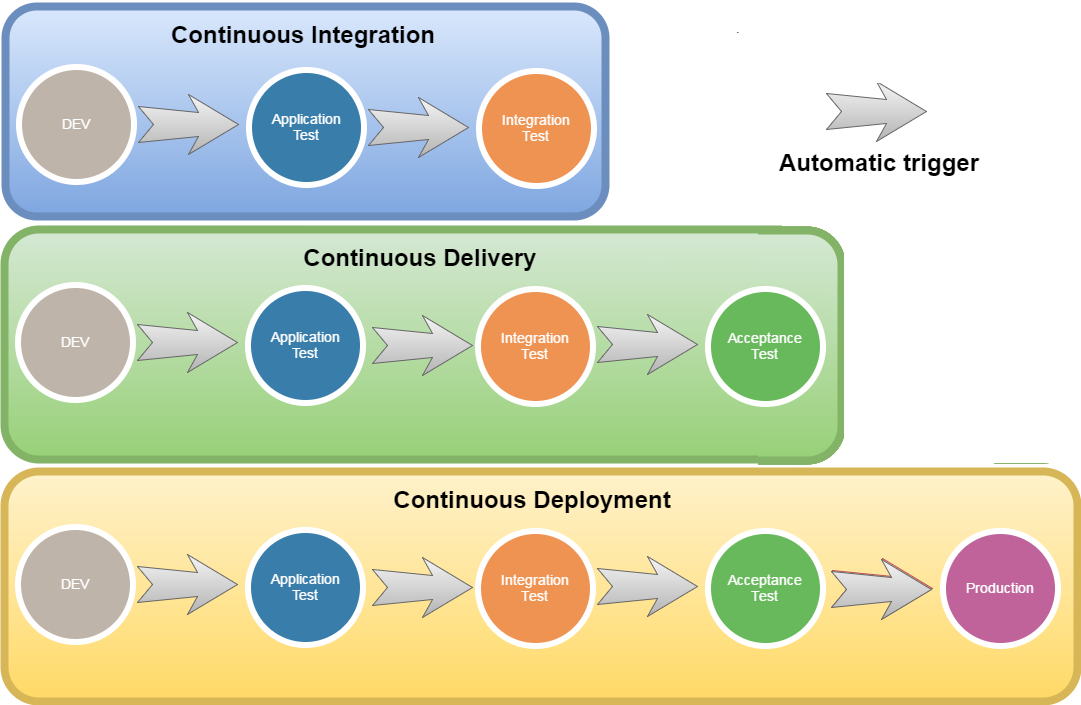
\includegraphics[width=\linewidth]{CI-CD}
  \caption{Continious integration}
  \label{fig:CI-CD}
  \end{center}
\end{figure}

\newpage

\begin{figure}[h]
  \begin{center}
  
\includegraphics[width=0.8\linewidth]{lockScreen}
  \caption{Ecran verrouillé}
  \label{fig:lockScreen}
\end{center}
\end{figure}

\begin{figure}[h]
  \begin{center}
  
\includegraphics[width=0.8\linewidth]{tryUnlockScreen}
  \caption{Déverrouillage écran avec reconnaissance faciale}
  \label{fig:tryUnlockScreen}
\end{center}
\end{figure}

\begin{figure}[h]
  \begin{center}
  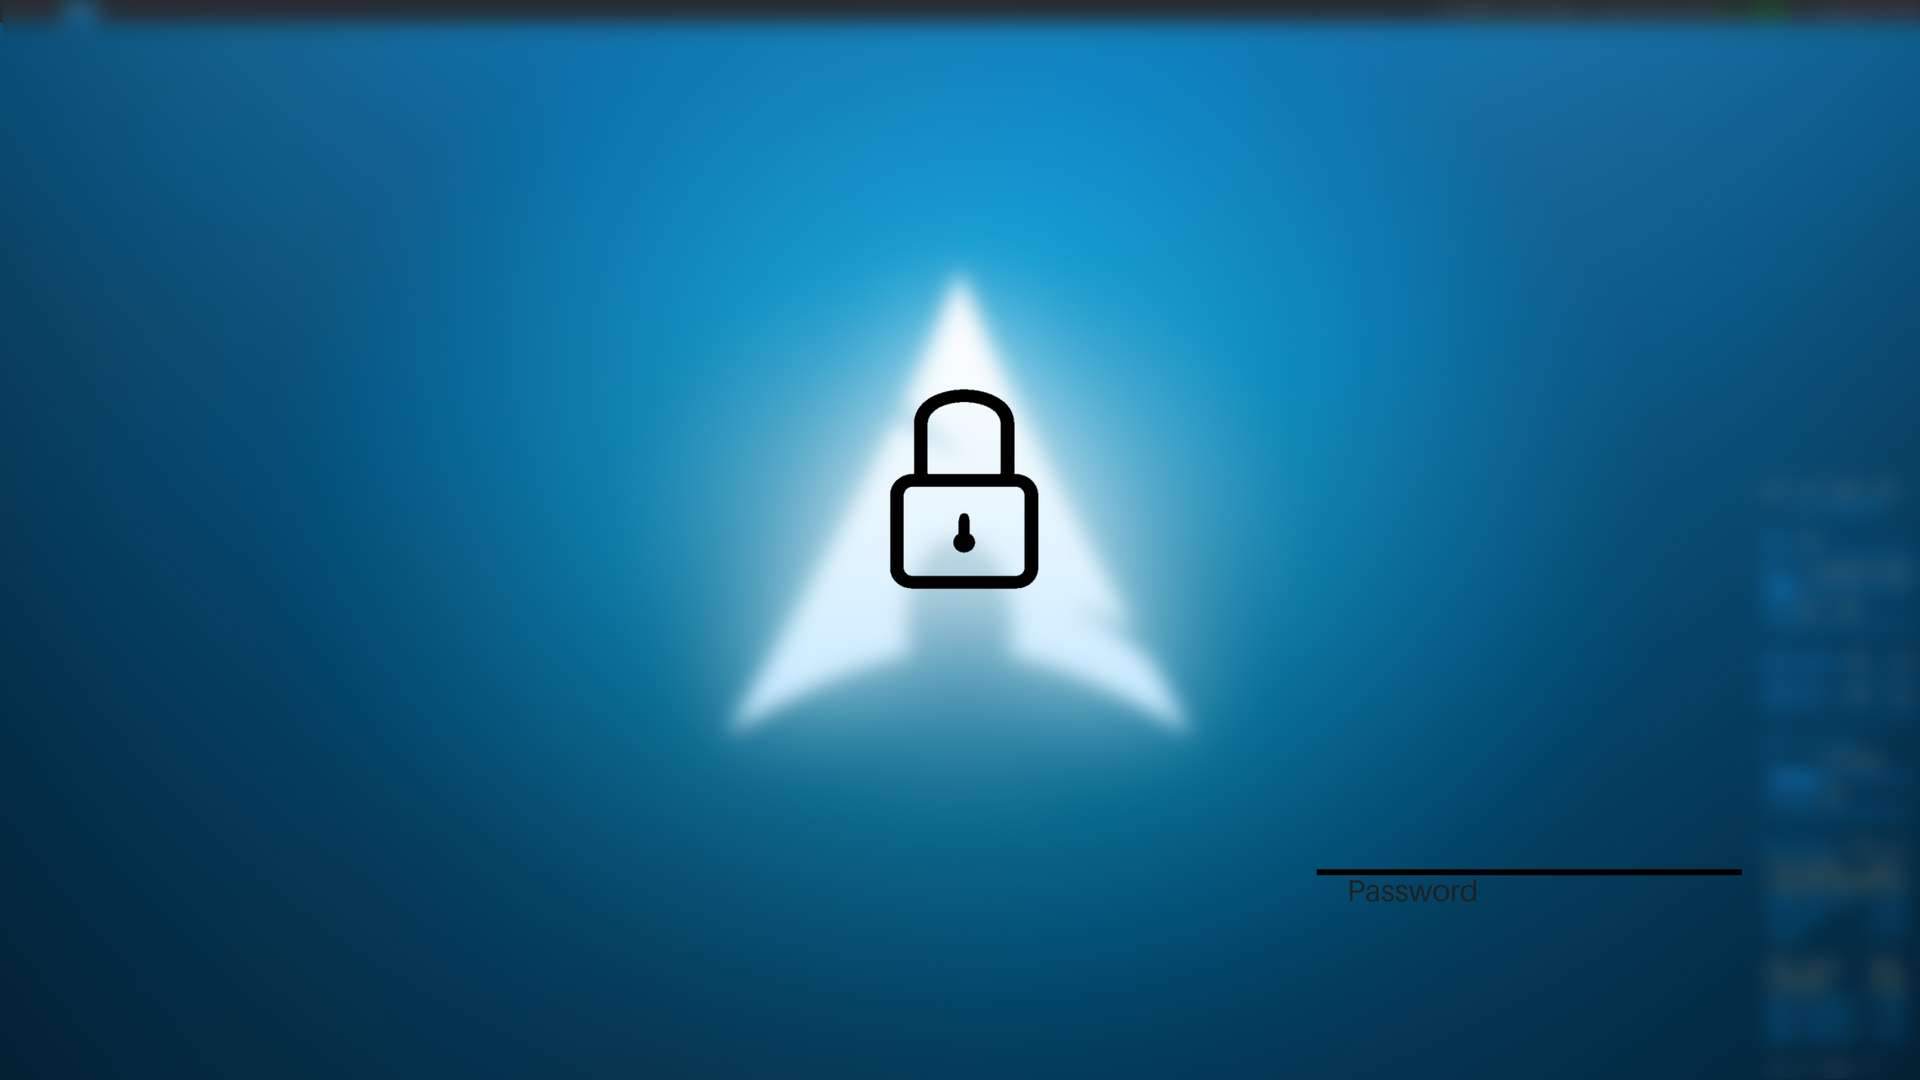
\includegraphics[width=\linewidth]{passwordScreen}
  \caption{Déverrouillage écran, demande mot de passe}
  \label{fig:passwordScreen}
\end{center}
\end{figure}

\begin{figure}[h]
  \begin{center}
  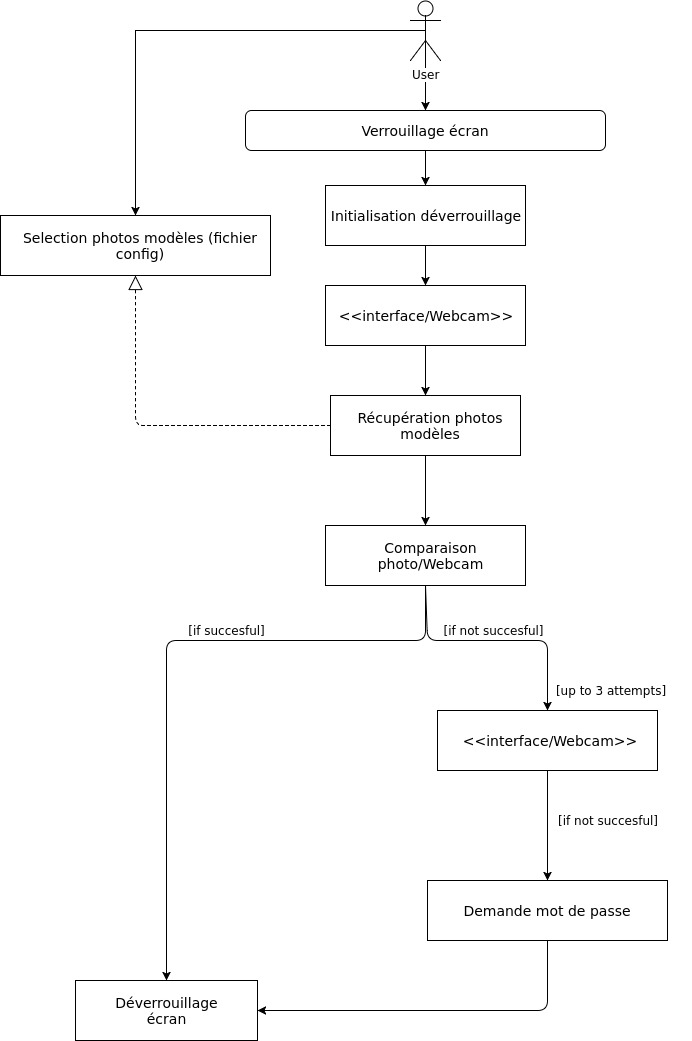
\includegraphics[width=0.75\linewidth]{Organisation}
  \caption{Diagramme explication du fonctionnement général de lockatme}
\end{center}
\end{figure}

\begin{figure}[h]
  \begin{center}
  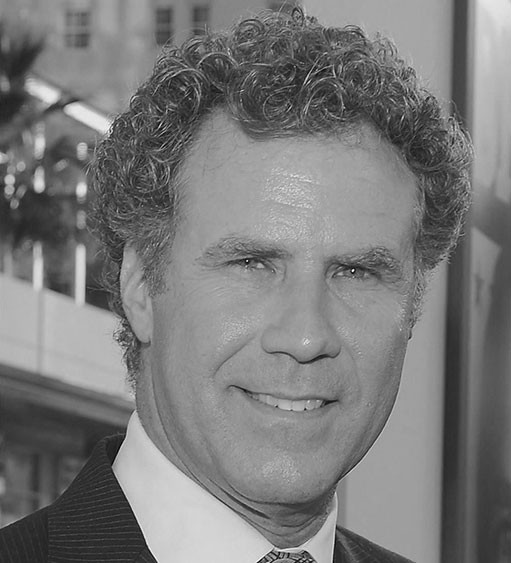
\includegraphics[width=0.4\linewidth]{HOG1}
  \caption{Exemple représentation HOG (1)}
  \label{fig:HOG}
\end{center}
\end{figure}

\begin{figure}[h]
  \begin{center}
  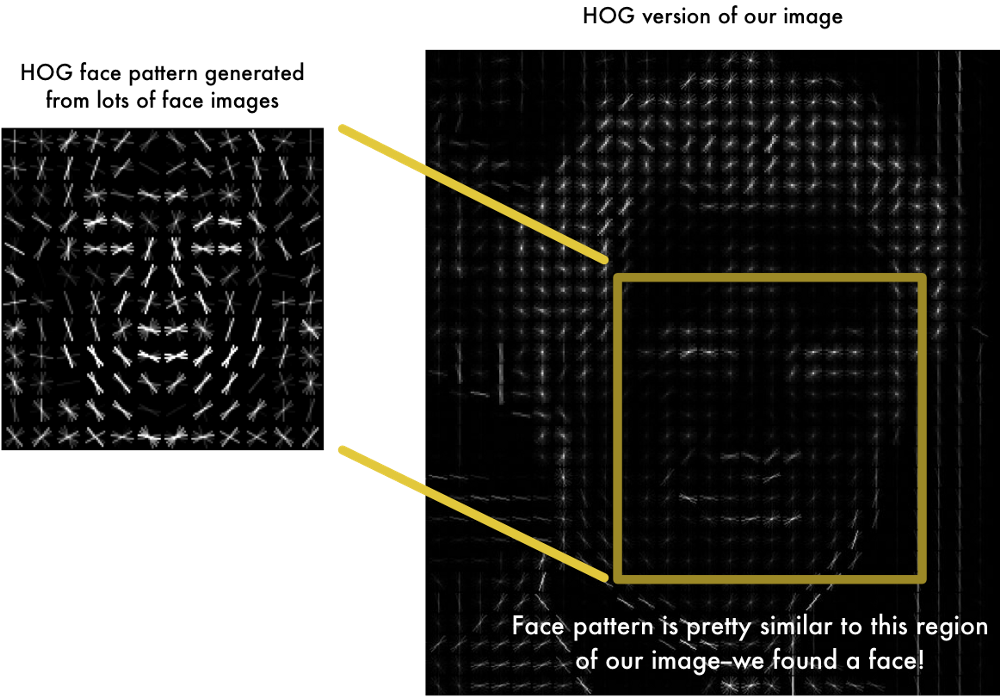
\includegraphics[width=0.7\linewidth]{HOG}
  \caption{Exemple représentation HOG (2)}
  \label{fig:HOG1}
\end{center}
\end{figure}

\begin{figure}[h]
  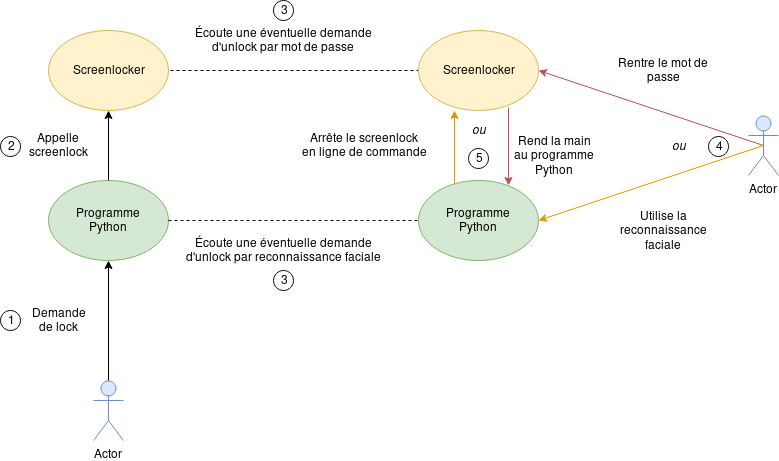
\includegraphics[width=\linewidth]{diagramme_lockatme}
  \caption{Diagramme appel programme tiers}
  \label{fig:dialam}
\end{figure}


\chapter{Code}
\newpage
\begin{minted}{python}
import face_recognition
import cv2
video_capture = cv2.VideoCapture(0)
juju_image = face_recognition.load_image_file("juju.jpg")
pl_image = face_recognition.load_image_file("pl.jpg")

juju_face_encoding = face_recognition.face_encodings(juju_image)[0]
pl_face_encoding = face_recognition.face_encodings(pl_image)[0]

while True:
     ret, frame = video_capture.read()

     face_locations = face_recognition.face_locations(frame)
     face_encodings = face_recognition.face_encodings(frame, face_locations)

     for (top, right, bottom, left), face_encoding in zip(face_locations,
       face_encodings):
          #See if the face is a match for the known face(s)
          match = face_recognition.compare_faces([juju_face_encoding],
            face_encoding)
          match1 = face_recognition.compare_faces([pl_face_encoding],
            face_encoding)
          name = "Unknown"
          if match[0]:
               name = "Juliette"
          if match1[0]:
              name = "PL"
          #Draw a box around the face
          cv2.rectangle(frame, (left, top), (right, bottom), (0, 0, 255), 2)

          #Draw a label with a name below the face
          cv2.rectangle(frame, (left, bottom - 35), (right, bottom), (0, 0,
            255), cv2.FILLED)
          font = cv2.FONT_HERSHEY_DUPLEX
          cv2.putText(frame, name, (left + 6, bottom - 6), font, 1.0, (255,
            255, 255), 1)

     #Display the resulting image
     cv2.imshow('Video', frame)

     #Hit 'q' on the keyboard to quit!
     if cv2.waitKey(1) & 0xFF == ord('q'):
          break
#Release handle to the webcam
video_capture.release()
cv2.destroyAllWindows()
\end{minted}
